\documentclass[14pt]{beamer}

\mode<presentation>{ \usetheme{Madrid}

% To remove the navigation symbols from the bottom of all slides uncomment next line
\setbeamertemplate{navigation symbols}{}
\date{}
\title{}
\author{}

%to get rid of footer entirely uncomment next line
\setbeamertemplate{footline}{}
}

\usepackage{geometry}
\usepackage{multirow}
\usepackage{adjustbox}
\usepackage{multicol}
\setlength{\columnsep}{0.1cm}

\usepackage{tikz}
\usetikzlibrary{shapes, backgrounds}

\usepackage{bbding}
\usepackage{rotating}
\usepackage{xcolor}

\usepackage{tkz-berge} %cool grid
\usepackage{pgfplots} %pics

\usepackage{graphicx} % Allows including images
\usepackage{
	booktabs
} % Allows the use of \toprule, \midrule and \bottomrule in tables
\usepackage{mathtools}

\newcommand{\R}{\mathbb{R}}
\newcommand{\Z}{\mathbb{Z}}
\newcommand{\N}{\mathbb{N}}
\newcommand{\e}{\varepsilon}

\newcommand{\p}{% \pause
}

% simple environrment for enumerate, easier to read
\setbeamertemplate{enumerate items}[default]

%%%%%%%%%%%%%%%%%%%%%%

% to use colours easily
\definecolor{miverde}{rgb}{0.7, .5, 0.7}
\newcommand{\azul}[1]{{\color{blue} #1}}
\newcommand{\rojo}[1]{{\color{red} #1}}
\newcommand{\verde}[1]{{\color{miverde} #1}}

% box in red and blue in math and outside of math
\newcommand{\cajar}[1]{\boxed{\mbox{\rojo{ #1}}}}
\newcommand{\majar}[1]{\boxed{\rojo{ #1}}}
\newcommand{\cajab}[1]{\boxed{\mbox{\azul{ #1}}}}
\newcommand{\majab}[1]{\boxed{\azul{ #1}}}

\newcommand{\setsize}[1]{\fontsize{#1}{#1}\selectfont} %allows you to change the font size. The default size of this document is 14. To change the font size of the whole slide, place this at the beginning of the slide. To change the size of only a portion of the text to size 12, you can do the following { \setsize{12} Your text. }.

\setbeamerfont{frametitle}{size=\fontsize{15}{15}\selectfont}
\setbeamerfont{block title}{size=\fontsize{14}{14}\selectfont}

\newcommand{\smallerfont}{\setsize{13}} %place this at the beginning of a slide to set the font size of the entire slide to 13.

%===========================

%===================================================
\begin{document}
	%===================================================

	%----------------------------------------------------------------------------------------

	%	CLASS QUESTIONS

	%----------------------------------------------------------------------------------------

	%------------------------------

	%QUESTION_INFO: {"unit":1,"question":0,"title":"Warm-up","images":[]}
	\begin{frame}
		\frametitle{Warm-up}

		What are the following sets?

		\begin{enumerate}
			\item $[2,4] \cup (2,5)$

			\item $[2,4] \cap (2,5)$

			\item $[\pi,e]$

			\item $[0,0]$

			\item $(0,0)$
		\end{enumerate}
	\end{frame}

	%-----------------------------

	%QUESTION_INFO: {"unit":1,"question":1,"title":"Similar sets","images":[]}
	\begin{frame}
		\frametitle{Similar sets}

		What are the following sets?

		\begin{enumerate}
			\item $\displaystyle A = \{ x \in \mathbb{Z}: x^{2}< 6\}$

			\item $\displaystyle B = \{ x \in \mathbb{N}: x^{2}< 6\}$

			\item $\displaystyle C = \{ x \in \mathbb{R}: x^{2}< 6\}$
		\end{enumerate}
	\end{frame}

	%-----------------------------

	%QUESTION_INFO: {"unit":1,"question":2,"title":"Describing a new set","images":[]}
	\begin{frame}
		\frametitle{Describing a new set}

		An irrational number is a number that is real but not rational.

		$B$ is the set of positive, rational numbers and negative, irrational
		numbers.

		Write a definition for $B$ using only mathematical notation. \\ (You may use
		the words ``and", ``or", and ``such that".)
	\end{frame}

	%-----------------------------

	%QUESTION_INFO: {"unit":1,"question":3,"title":"Sets and quantifiers","images":[]}
	\begin{frame}
		\frametitle{Sets and quantifiers}

		What are the following sets?

		\begin{enumerate}
			\item $\displaystyle A = \{ x \in \mathbb{R}\, : \, \forall y \in [0,1], \,
				x < y \}$

			\item $\displaystyle B = \{ x \in \mathbb{R}\, : \, \exists y \in [0,1] \text{
				s.t. }x < y \}$

			\item $\displaystyle C = \{ x \in [0,1] \, : \, \forall y \in [0,1], x < y
				\}$

			\item $\displaystyle D = \{ x \in [0,1] \, : \, \exists y \in [0,1] \text{
				s.t. }x < y \}$

			\item $\displaystyle E = \{ x \in [0,1] \, : \, \exists y \in \mathbb{R}\text{
				s.t. }x < y \}$

			\item $\displaystyle F = \{ x \in [0,1] \, : \, y \in \mathbb{R}, \, x < y
				\}$
		\end{enumerate}
	\end{frame}

	%-----------------------------

	%QUESTION_INFO: {"unit":1,"question":4,"title":"Functions and quantifiers","images":[]}
	\begin{frame}
		\frametitle{Functions and quantifiers}

		Let $f$ be a function with domain $\mathbb{R}$. Rewrite the following statements
		using $\forall$ or $\exists$:

		\begin{enumerate}
			\item The graph of $f$ intercepts the $x$-axis.

			\item $f$ is the zero function.

			\item $f$ is not the zero function.

			\item $f$ never vanishes.

			\item The equation $\displaystyle f(x)=0$ has a solution.

			\item The equation $\displaystyle f(x)=0$ has no solutions.

			\item $f$ takes both positive and negative values.

			\item $f$ is never negative.
		\end{enumerate}
	\end{frame}

	%------------------------------

	%QUESTION_INFO: {"unit":1,"question":5,"title":"Negation 1","images":[]}
	\begin{frame}
		\frametitle{Negation 1}

		Write the negation of these statements as simply as possible:

		\begin{enumerate}
			\item My favourite integer number is greater than $7$.

			\item I know at least five students at U of T who have a cellphone.

			\item There is a country in the European Union with fewer than 1000 inhabitants.

			\item All of my friends like apples.

			\item I like apples and oranges.
		\end{enumerate}

		\vfill

		\begin{center}
			Negation of $\displaystyle \boxed{{\color{blue} \cdots}}$ \; = \; $\displaystyle
			\boxed{{\color{blue} \cdots}}$ is false.
		\end{center}
	\end{frame}

	%-----------------------------

	%QUESTION_INFO: {"unit":1,"question":6,"title":"Negation 2","images":[]}
	\begin{frame}
		\frametitle{Negation 2}

		Write the negation of this statement without using any negative words (``no",
		``not", ``none", etc.):

		\begin{quote}
			``\emph{Every page in this book contains at least one word whose first and
			last letters both come alphabetically before M.}''
		\end{quote}
	\end{frame}

	%-----------------------------

	%QUESTION_INFO: {"unit":1,"question":7,"title":"Negation 3","images":[]}
	\begin{frame}
		\frametitle{Negation 3}

		Negate the following statement without using any negative words (``no", ``not",
		``none", etc.):

		\begin{quote}
			``\emph{I have a friend all of whose former boyfriends had at least two
			siblings with exactly three different vowels in their name.}''
		\end{quote}
	\end{frame}

	%-----------------------------

	%QUESTION_INFO: {"unit":1,"question":8,"title":"Symmetric difference","images":[]}
	\begin{frame}
		\frametitle{Symmetric difference}

		Given two sets $A$ and $B$, we define
		\begin{itemize}
			\item $A \setminus B = \{ x \in A \; : \; x \notin B \}$

			\item $A \triangle B = (A \setminus B) \cup (B \setminus A)$
		\end{itemize}

		\vfill

		Let
		\begin{itemize}
			\item $C_{1}= \{ \text{ students under 18 }\}$

			\item $C_{2}= \{ \text{ students born in Ontario }\}$
		\end{itemize}

		\vfill

		What is the set $C_{1}\triangle C_{2}$?

		\vfill
	\end{frame}
	%-----------------------------

	%QUESTION_INFO: {"unit":1,"question":9,"title":"Symmetric difference - 2","images":[]}
	\begin{frame}
		\frametitle{Symmetric difference - 2}

		Given two sets $A$ and $B$, we define
		\begin{itemize}
			\item $A \setminus B = \{ x \in A \; : \; x \notin B \}$

			\item $A \triangle B = (A \setminus B) \cup (B \setminus A)$
		\end{itemize}

		\vfill

		Is the following equality
		\[
			(A \triangle B) \triangle C \; = \; A \triangle (B \triangle C)
		\]
		true for all sets $A$, $B$, and $C$?

		\vfill
	\end{frame}
	%------------------------------

	%QUESTION_INFO: {"unit":1,"question":10,"title":"Even numbers","images":[]}
	\begin{frame}[t]
		\frametitle{Even numbers}

		Write a description of the set $E$ of even integers using set-building
		notation.
	\end{frame}

	%------------------------------

	%QUESTION_INFO: {"unit":1,"question":11,"title":"Even numbers","images":[]}
	\begin{frame}[t]
		\frametitle{Even numbers}

		Which of these is a correct description of the set $E$ of even integers?
		\begin{enumerate}
			\item $\displaystyle E = \{ n \in \mathbb{Z}\; : \; \forall a \in \mathbb{Z}
				, \, n = 2a \}$

			\item $\displaystyle E = \{ n \in \mathbb{Z}\; : \; \exists a \in \mathbb{Z}
				\text{ s.t. }n = 2a \}$
		\end{enumerate}

		\vfill
		% \pause

		Which of these statements is true?
		\begin{enumerate}
			\addtocounter{enumi}{2}

			\item $\displaystyle \forall a \in \mathbb{Z}$, the number
				$\displaystyle n=2a$ is even.

			\item $\displaystyle \exists a \in \mathbb{Z}$ s.t. the number
				$\displaystyle n=2a$ is even.
		\end{enumerate}

		\vfill
	\end{frame}

	%-----------------------------

	%QUESTION_INFO: {"unit":1,"question":12,"title":"Mother","images":[]}
	\begin{frame}
		\frametitle{Mother}

		Let
		\[
			H = \{ \text{ humans }\}
		\]

		\vfill

		True or False?

		\begin{enumerate}
			\item $\displaystyle \forall x \in H, \; \exists y \in H$ \mbox{ such that
				} $y$ gave birth to $x$

			\item $\displaystyle \exists y \in H \text{ such that }\forall x \in H$,
				$y$ gave birth to $x$
		\end{enumerate}

		\vfill
	\end{frame}

	%----------------------------

	%QUESTION_INFO: {"unit":1,"question":13,"title":"Elephants","images":[]}
	\begin{frame}
		\frametitle{Elephants}

		True or False?

		\begin{enumerate}
			\item There is a pink elephant in this room.

			\item All elephants in this room are pink.
		\end{enumerate}
	\end{frame}
	%-----------------------------

	%QUESTION_INFO: {"unit":1,"question":14,"title":"Indecisive function","images":[]}
	\begin{frame}
		\frametitle{Indecisive function}

		Construct a function $f$ that satisfies all of the following properties at
		once:
		\begin{itemize}
			\item The domain of $f$ is $\mathbb{R}$.

			\item $\displaystyle \forall x \in \mathbb{R}, \exists y \in \mathbb{R}$ such
				that
				\[
					x<y \text{ and }f(x) < f(y)
				\]

			\item $\displaystyle \forall x \in \mathbb{R}, \exists y \in \mathbb{R}$ such
				that
				\[
					x<y \text{ and }f(x) > f(y)
				\]
		\end{itemize}
	\end{frame}
	%-----------------------------

	%QUESTION_INFO: {"unit":1,"question":15,"title":" Conditionals - True or False?","images":[]}
	\begin{frame}
		\frametitle{ Conditionals - True or False?}

		Let $\displaystyle x \in \mathbb{R}$.

		\begin{enumerate}
			\item $\displaystyle x > 0 \quad \implies \quad x \geq 0$

			\item $\displaystyle x \geq 0 \quad \implies \quad x > 0$

				\vfill
			% \pause

			\item IF $\displaystyle 2 > 3$ THEN Alfonso is in love.
		\end{enumerate}

		\vfill
	\end{frame}
	%-----------------------------

	%QUESTION_INFO: {"unit":1,"question":16,"title":"Negation of conditionals","images":[]}
	\begin{frame}
		\frametitle{Negation of conditionals}

		Write the negation of these statements:
		\begin{enumerate}
			\item If Justin Trudeau has a brother, then he also has a sister.

			\item If a student in this class has a brother, then they also have a
				sister.
		\end{enumerate}
	\end{frame}

	%------------------------------

	%QUESTION_INFO: {"unit":1,"question":17,"title":"Cards","images":[]}
	\begin{frame}
		\frametitle{Cards}

		Take a look at the following cards.

		\begin{center}
			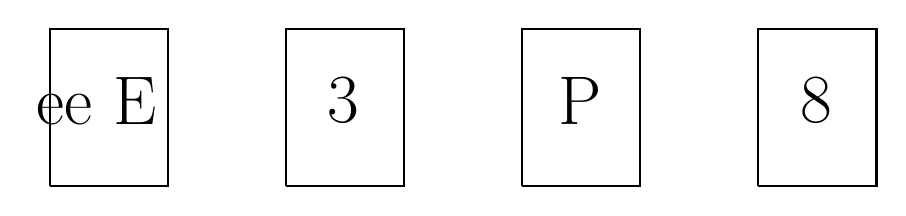
\begin{tikzpicture}
				\draw[thick] (0,0) -- (0,2) -- (1.5,2) -- (1.5,0) -- (0,0);
				\draw[thick] (3,0) -- (3,2) -- (4.5,2) -- (4.5,0) -- (3,0);
				\draw[thick] (6,0) -- (6,2) -- (7.5,2) -- (7.5,0) -- (6,0);
				\draw[thick] (9,0) -- (9,2) -- (10.5,2) -- (10.5,0) -- (9,0);
				\node[below] at (0.6,1.5) {\Huge{\hyperlink{ee}{{ E}} }};
				\node[below] at (3.6,1.5) {\Huge{ 3}};
				\node[below] at (6.6,1.5) {\Huge{ P}};
				\node[below] at (9.6,1.5) {\Huge{ 8}};
			\end{tikzpicture}
		\end{center}

		Each card has a letter on one side and a number on the other, and I tell you:

		\medskip
		\begin{block}{}
			\emph{``\textbf{If} a card has a vowel on one side, \\ \textbf{then} it has
			an odd number on the other side." }
		\end{block}

		\medskip
		Which cards do you need to turn over in order to verify whether I am telling
		the truth or not?

		%

		%

		%%%\Large

		%

		%Four cards lie on the table in front of you.  You know that each card has a letter on one side and a number on the other.  At the moment, you can read the symbols $E$, $P$, $3$, and $8$ on the sides that are up.  I tell you:

		%

		%\vfill

		%

		%\begin{block}{}

		%		 \emph{``\textbf{If} a card has a vowel on one side, \\

		%		 \textbf{then} it has an odd number on the other side." }

		%\end{block}

		%

		%\vfill

		%

		%Which cards do you need to turn over in order to verify whether I am telling the truth or not?
	\end{frame}

	%------------------------------

	%QUESTION_INFO: {"unit":1,"question":18,"title":"Cards - 2","images":[]}
	\begin{frame}
		\frametitle{Cards - 2}

		Four cards lie on the table in front of you. You know that each card has a letter
		on one side and a number on the other.

		{\bfseries Negate} the following statement:
		\begin{block}{}
			\emph{``\textbf{If} a card has a vowel on one side, \\ \textbf{then} it has
			an odd number on the other side." }
		\end{block}
	\end{frame}

	%-----------------------------

	%QUESTION_INFO: {"unit":1,"question":19,"title":"Hockey","images":[]}
	\begin{frame}
		\frametitle{Hockey}

		Which of the following statements are equivalent to the statement \quad
		\emph{``Every Canadian man likes hockey''}?

		\begin{enumerate}
			\item If a man is Canadian, then he likes hockey.

			\item If a man likes hockey, then he is Canadian.

			\item If a man does not like hockey, then he is not Canadian.

			\item If a man is not Canadian, then he likes hockey.

			\item Non-Canadian men do not like hockey.

			\item If a Canadian does not like hockey, then she is not a man.
		\end{enumerate}
	\end{frame}

	%-----------------------------

	%QUESTION_INFO: {"unit":1,"question":20,"title":"Graphs","images":[]}
	\begin{frame}
		\frametitle{Graphs}

		Draw the graph of a function $f$ with domain $\mathbb{R}$ that satisfies:
		\begin{equation*}
			\text{If }2<x<4 \text{ then }1<f(x)<2.
		\end{equation*}
		\vfill

		Draw the graph of a function $g$ with domain $\mathbb{R}$ that satisfies:
		\begin{equation*}
			2<x<4 \text{ if and only if }1 < g(x) < 2.
		\end{equation*}
		\vfill
	\end{frame}

	%------------------------------

	%QUESTION_INFO: {"unit":1,"question":21,"title":"One-to-one functions","images":[]}
	\begin{frame}
		\frametitle{One-to-one functions}

		Let $f$ be a function with domain $D$. \\

		\vfill

		$f$ is \emph{one-to-one} means that ...
		\begin{itemize}
			\item ... different inputs (${\color{red} x}$) ...

			\item ... must produce different outputs (${\color{red} f(x)}$).
		\end{itemize}

		% \pause
		\vfill

		\begin{block}{}
			Write a formal definition of ``one-to-one".
		\end{block}
	\end{frame}

	%-----------------------------

	%QUESTION_INFO: {"unit":1,"question":22,"title":"One-to-one functions","images":[]}
	\begin{frame}
		\frametitle{One-to-one functions}

		{\bfseries Definition:} Let $f$ be a function with domain $D$. \\ $f$ is one-to-one
		means ...
		\begin{enumerate}
			\item $\displaystyle f(x_{1}) \neq f(x_{2})$

			\item $\displaystyle \exists x_{1}, x_{2}\in D, \; f(x_{1}) \neq f(x_{2})$

			\item $\displaystyle \forall x_{1}, x_{2}\in D, \; f(x_{1}) \neq f(x_{2})$

			\item $\displaystyle \forall x_{1}, x_{2}\in D, \; x_{1}\neq x_{2}, \; f(x_{1}
				) \neq f(x_{2})$

			\item $\displaystyle \forall x_{1}, x_{2}\in D, \; x_{1}\neq x_{2}\implies
				f(x_{1}) \neq f(x_{2})$

			\item $\displaystyle \forall x_{1}, x_{2}\in D, \; f(x_{1}) \neq f(x_{2}) \implies
				x_{1}\neq x_{2}$

			\item $\displaystyle \forall x_{1}, x_{2}\in D, \; f(x_{1}) = f(x_{2}) \implies
				x_{1}= x_{2}$
		\end{enumerate}
	\end{frame}

	%-----------------------------

	%QUESTION_INFO: {"unit":1,"question":23,"title":"One-to-one functions","images":[]}
	\begin{frame}
		\frametitle{One-to-one functions}

		Let $f$ be a function with domain $D$. \\ {\bfseries What does each of the following mean?}
		\begin{enumerate}
			\item $\displaystyle f(x_{1}) \neq f(x_{2})$

			\item $\displaystyle \exists x_{1}, x_{2}\in D, \; f(x_{1}) \neq f(x_{2})$

			\item $\displaystyle \forall x_{1}, x_{2}\in D, \; f(x_{1}) \neq f(x_{2})$

			\item $\displaystyle \forall x_{1}, x_{2}\in D, \; x_{1}\neq x_{2}, \; f(x_{1}
				) \neq f(x_{2})$

			\item $\displaystyle \forall x_{1}, x_{2}\in D, \; x_{1}\neq x_{2}\implies
				f(x_{1}) \neq f(x_{2})$

			\item $\displaystyle \forall x_{1}, x_{2}\in D, \; f(x_{1}) \neq f(x_{2}) \implies
				x_{1}\neq x_{2}$

			\item $\displaystyle \forall x_{1}, x_{2}\in D, \; f(x_{1}) = f(x_{2}) \implies
				x_{1}= x_{2}$
		\end{enumerate}
	\end{frame}
	%-----------------------------

	%QUESTION_INFO: {"unit":1,"question":24,"title":"Proving a function is one-to-one","images":[]}
	\begin{frame}
		\frametitle{Proving a function is one-to-one}
		\fontsize{13}{13}\selectfont

		\begin{block}{Definition}
			Let $f$ be a function with domain $D$. \\ We say $f$ is one-to-one when
			\begin{itemize}
				\item \hfill $\displaystyle \forall x_{1}, x_{2}\in D, \; x_{1}\neq x_{2}
					\implies f(x_{1}) \neq f(x_{2})$

				\item OR, equivalently, \hfill $\displaystyle \forall x_{1}, x_{2}\in D,
					\; f(x_{1}) = f(x_{2}) \implies x_{1}= x_{2}$
			\end{itemize}
		\end{block}

		\vfill
		% \pause

		Suppose I give you a specific function $f$ and I ask you to prove it is one-to-one.
		% \pause
		\begin{itemize}
			\item Write the structure of your proof (how do you begin? what do you assume?
				what do you conclude?) if you use the first definition.

			\item Write the structure of your proof if you use the second definition.
		\end{itemize}

		\vfill
		% \pause

		\begin{block}{Exercise}
			Prove that $f(x) = 3x + 2$, with domain $\mathbb{R}$, is one-to-one.
		\end{block}
	\end{frame}

	%-----------------------------

	%QUESTION_INFO: {"unit":1,"question":25,"title":"Proving a function is NOT one-to-one","images":[]}
	\begin{frame}[t]
		\fontsize{13}{13}\selectfont
		\frametitle{Proving a function is NOT one-to-one}

		\begin{block}{Definition}
			Let $f$ be a function with domain $D$. \\ We say $f$ is one-to-one when
			\begin{itemize}
				\item \hfill $\displaystyle \forall x_{1}, x_{2}\in D, \; x_{1}\neq x_{2}
					\implies f(x_{1}) \neq f(x_{2})$

				\item OR, equivalently, \hfill $\displaystyle \forall x_{1}, x_{2}\in D,
					\; f(x_{1}) = f(x_{2}) \implies x_{1}= x_{2}$
			\end{itemize}
		\end{block}

		\vfill
		% \pause

		Suppose I give you a specific function $f$ and I ask you to prove it is not one-to-one.
		% \pause
		You need to prove $f$ satisfies the \emph{negation} of the definition.
		\begin{itemize}
			\item Write the negation of the first definition.

			\item Write the negation of the second definition.

			\item Write the structure of your proof.
		\end{itemize}

		\vfill
		% \pause

		\begin{block}{Exercise}
			Prove that $f(x) = x^{2}$, with domain $\mathbb{R}$, is not one-to-one.
		\end{block}
	\end{frame}

	%-----------------------------

	%QUESTION_INFO: {"unit":1,"question":26,"title":"Proving a theorem","images":[]}
	\begin{frame}
		\frametitle{Proving a theorem}

		\begin{block}{Theorem}
			Let $f$ be a function with domain $D$.
			\begin{itemize}
				\item IF $f$ is increasing on $\displaystyle D$

				\item THEN $f$ is one-to-one on $\displaystyle D$
			\end{itemize}
		\end{block}

		\vfill
		% \pause

		\begin{enumerate}
			\item Remind yourself of the precise definition of ``increasing" and ``one-to-one".
			% \pause

			\item To prove the theorem, what will you assume? what do you want to show?
			% \pause

			\item Look at the part you want to show. Based on the definition, what is the
				structure of the proof?
			% \pause

			\item Complete the proof.
		\end{enumerate}
	\end{frame}

	%-----------------------------

	%QUESTION_INFO: {"unit":1,"question":27,"title":"DISproving a theorem","images":[]}
	\begin{frame}
		\frametitle{DISproving a theorem}

		\begin{block}{ FALSE Theorem}
			Let $f$ be a function with domain $D$.
			\begin{itemize}
				\item IF $f$ is one-to-one on $\displaystyle D$

				\item THEN $f$ is increasing on $\displaystyle D$
			\end{itemize}
		\end{block}

		\vfill
		% \pause

		\begin{enumerate}
			\item This theorem is false. What do you need to do to prove it is false?
			% \pause

			\item Prove the theorem is false.
		\end{enumerate}
	\end{frame}

	%-----------------------------

	%QUESTION_INFO: {"unit":1,"question":28,"title":"What is wrong with this proof? (1)","images":[]}
	\begin{frame}
		\frametitle{What is wrong with this proof? (1)}

		\begin{block}{Theorem}
			The sum of two odd numbers is even.
		\end{block}

		% \pause
		\vfill

		\begin{proof}
			3 is odd. \\ 5 is odd. \\ $3+5 = 8$ is even.
		\end{proof}

		\vfill
	\end{frame}
	%-----------------------------

	%QUESTION_INFO: {"unit":1,"question":29,"title":"What is wrong with this proof? (2)","images":[]}
	\begin{frame}
		\frametitle{What is wrong with this proof? (2)}

		\begin{block}{Theorem}
			The sum of two odd numbers is even.
		\end{block}

		% \pause
		\vfill

		\begin{proof}
			The sum of two odd numbers is always even. \\ even + even = even \\ even +
			odd = odd \\ odd + even = odd \\ odd + odd = even.
		\end{proof}

		\vfill
	\end{frame}
	%-----------------------------

	%QUESTION_INFO: {"unit":1,"question":30,"title":"Definition of odd and even","images":[]}
	\begin{frame}
		\frametitle{Definition of odd and even}

		Write a definition of ``odd integer" and ``even integer".

		% \pause
		\vfill

		\begin{block}{Definition}
			Let $x \in \mathbb{Z}$. We say that $x$ is odd when ...
			\begin{enumerate}
				\item $x = 2a+1$ ?

				\item $\displaystyle \forall a \in \mathbb{Z}, x = 2a+ 1$?

				\item $\displaystyle \exists a \in \mathbb{Z}\text{ s.t. }x = 2a+ 1$?
			\end{enumerate}
		\end{block}

		\vfill
	\end{frame}

	%-----------------------------

	%QUESTION_INFO: {"unit":1,"question":31,"title":"What is wrong with this proof? (3)","images":[]}
	\begin{frame}
		\frametitle{What is wrong with this proof? (3)}

		\begin{block}{Theorem}
			The sum of two odd numbers is always even.
		\end{block}

		% \pause

		\begin{proof}
			$\displaystyle x= 2a + 1$ odd

			$\displaystyle y = 2b + 1$ odd

			$\displaystyle x+ y = 2n$ even

			$\displaystyle 2a + 1 + 2b + 1 = 2n$

			$\displaystyle 2a + 2b + 2 = 2n$

			$\displaystyle a + b + 1 = n$
		\end{proof}
	\end{frame}

	%-----------------------------

	%QUESTION_INFO: {"unit":1,"question":32,"title":"Write a correct proof!","images":[]}
	\begin{frame}
		\frametitle{Write a correct proof!}

		\begin{block}{Theorem}
			The sum of two odd numbers is always even.
		\end{block}
	\end{frame}

	%------------------------------

	%QUESTION_INFO: {"unit":1,"question":33,"title":"Variations on induction","images":[]}
	\begin{frame}
		\frametitle{Variations on induction}

		Let $S_{n}$ be a statement depending on a positive integer $n$.

		\vfill

		In each of the following cases, which statements are guaranteed to be true?

		\vfill
		% \pause

		\begin{multicols}{2}
			\begin{enumerate}
				\item We have proven:
					\begin{itemize}
						\item $S_{3}$

						\item $\displaystyle \forall n \geq 1, \; S_{n}\implies S_{n+1}$
					\end{itemize}

				\item We have proven:
					\begin{itemize}
						\item $S_{1}$

						\item $\displaystyle \forall n \geq 3, \; S_{n}\implies S_{n+1}$
					\end{itemize}

				\item We have proven:
					\begin{itemize}
						\item $S_{1}$

						\item $\displaystyle \forall n \geq 1, \; S_{n}\implies S_{n+3}$
					\end{itemize}

				\item We have proven:
					\begin{itemize}
						\item $S_{1}$

						\item $\displaystyle \forall n \geq 1, \; S_{n+1}\implies S_{n}$
					\end{itemize}
			\end{enumerate}
		\end{multicols}

		\vfill
	\end{frame}

	%-----------------------------

	%QUESTION_INFO: {"unit":1,"question":34,"title":"Variations on induction 2","images":[]}
	\begin{frame}
		\frametitle{Variations on induction 2}

		We want to prove
		\[
			\forall n \geq 1, \; S_{n}
		\]

		\vfill

		So far we have proven
		\begin{itemize}
			\item $S_{1}$

			\item $\displaystyle \forall n \geq 1, \; S_{n}\implies S_{n+3}.$
		\end{itemize}

		\vfill

		What else do we need to do?
	\end{frame}

	%-----------------------------

	%QUESTION_INFO: {"unit":1,"question":35,"title":"Variations on induction 3","images":[]}
	\begin{frame}
		\frametitle{Variations on induction 3}

		We want to prove
		\[
			\forall n \in \mathbb{Z}, \; S_{n}
		\]

		\vfill

		So far we have proven
		\begin{itemize}
			\item $S_{1}$
		\end{itemize}

		\vfill

		What else do we need to do?
	\end{frame}

	%----------------------------

	%QUESTION_INFO: {"unit":1,"question":36,"title":"What is wrong with this proof by induction?","images":[]}
	\begin{frame}
		\frametitle{What is wrong with this proof by induction?}
		\fontsize{13}{13}\selectfont

		\vspace{-1.5mm}
		\begin{theorem}
			$\forall N \geq 1$, every set of $N$ students in MAT137 will get the same
			grade.
		\end{theorem}
		% \pause
		\vspace{-1mm}

		\begin{proof}
			\begin{itemize}
				\item {\bfseries Base case.} It is clearly true for $N=1$.

				\item {\bfseries Induction step.} \\ Assume it is true for $N$. I'll
					show it is true for $N+1$. \\ Take a set of $N+1$ students. By
					induction hypothesis:
					\begin{itemize}
						\item The first $N$ students get the same grade.

						\item The last $N$ students get the same grade.
					\end{itemize}
					\[
						\mathrlap{\overbrace{\phantom{\bullet \quad \bullet \quad \cdots
						\quad \bullet \quad \bullet }}^{\text{Same grade}}}\bullet \quad \underbrace{\bullet
						\quad \bullet \quad \cdots \quad \bullet \quad \bullet}_{\text{Same
						grade}}
					\]
					Hence the $N+1$ students all get the same grade.
			\end{itemize}
		\end{proof}
	\end{frame}
	%----------------------------

	%QUESTION_INFO: {"unit":1,"question":37,"title":"What is wrong with this proof by induction?","images":[]}
	\begin{frame}
		\frametitle{What is wrong with this proof by induction?}

		For every $N \geq 1$, let
		\begin{center}
			\begin{tabular}{rcc}
				$\displaystyle S_{N}$ = & ``every set of $N$ students in MAT137 \\
				                        & will get the same grade"
			\end{tabular}
		\end{center}

		\vfill
		% \pause

		What did we actually prove in the previous page?

		\begin{itemize}
			\item $S_{1}$ \, ?

			\item $\displaystyle \forall N \geq 1$, \,
				$\displaystyle S_{N}\implies S_{N+1}$ \, ?
		\end{itemize}

		\vfill
	\end{frame}

	%------------------------------

	%------------------------------

	%-----------------------------
\end{document}
%-----------------------------

%-----------------------------

%-----------------------------